\documentclass[tikz]{standalone}
\usetikzlibrary{arrows.meta}
\begin{document}
	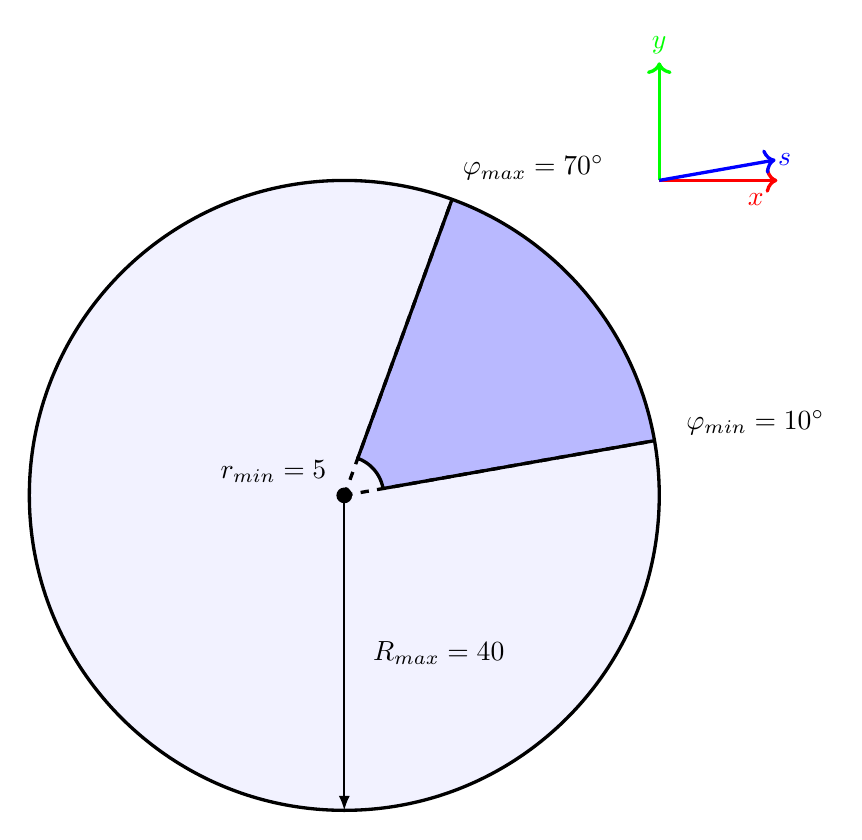
\begin{tikzpicture}
		
		\fill [blue!50, very nearly transparent] (0,0) circle (4);
		\fill [blue!50, semitransparent] ({0.5*cos(10)}, {0.5*sin(10)}) -- ({4*cos(10)}, {4*sin(10)}) arc (10:70:4) -- ({0.5*cos(70)}, {0.5*sin(70)}) arc (70:10:0.5);
		
		\draw [very thick](0,0) circle (4);
		\draw [very thick,domain=10:70] plot ({0.5*cos(\x)}, {0.5*sin(\x)});
		
		\draw [very thick] ({0.5*cos(10)}, {0.5*sin(10)}) -- (10:4);
		\draw [very thick, dashed] (0,0) -- (10:4);
		\draw [very thick] ({0.5*cos(70)}, {0.5*sin(70)}) -- (70:4);
		\draw [very thick, dashed] (0,0) -- (70:4);
		
		\draw [thick, -latex] (0,0) -- (0,-4);
		
		\fill [black] (0,0) circle (0.1);
		\node at (-0.9, 0.3) {$r_{min}=5$};		
		\node at (1.2, -2) {$R_{max}=40$};
		\node at (10:5.3) {$\varphi_{min}=10^\circ$};
		\node at (60:4.8) {$\varphi_{max}=70^\circ$};
		
		\draw[green,very thick, ->] (4,4) -- (4,5.5) node[above=-1]{$y$};
		\draw[red,very thick, ->] (4,4) -- (5.5,4) node[below left=1]{$x$};
		\draw [blue, very thick, ->] (4,4) -- ++(10:1.5) node[right=-3]{$s$};		
	\end{tikzpicture}
\end{document}